\documentclass{beamer}
\author{Shaun Schreiber (16715128)}
\title{Flow modeling and Cellular Automata}
\usetheme{Oxygen}
\usepackage{tikz,ifthen}
\date{\today}
\begin{document}
	\frame{\titlepage}
	%one
	\begin{frame}
	\frametitle{Outline}
    \tableofcontents[section=1,hidesubsections]
	\end{frame}

	%two
	\section{Lattice gas cellular automata}
	\begin{frame}
	\frametitle{Lattice gas cellular automata}
	\minipage{0.45\textwidth}
    \begin{block}{Basic structure}
    \begin{figure}[H]
  \centering
  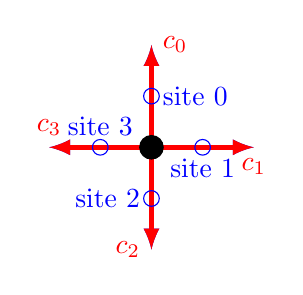
\begin{tikzpicture}[scale=0.65]

    \coordinate (Origin) at (0,0);
    \coordinate (site1) at (0,2);
    \coordinate (site2) at (2,0);
    \coordinate (site3) at (0,-2);
    \coordinate (site4) at (-2,0);  
    
    \draw [ultra thick,-latex,blue] (Origin)
        -- (site1) node [midway, right] {site 0};
    \draw [ultra thick,-latex,blue] (Origin)
        -- (site2) node [midway,below] {site 1};
    \draw [ultra thick,-latex,blue] (Origin)
        -- (site3) node [midway,left] {site 2};
    \draw [ultra thick,-latex,blue] (Origin)
        -- (site4) node [midway,above] {site 3};
        
	\draw [ultra thick,-latex,red] (Origin)
        -- (site1) node [right] {$c_0$};
    \draw [ultra thick,-latex,red] (Origin)
        -- (site2) node [below] {$c_1$};
    \draw [ultra thick,-latex,red] (Origin)
        -- (site3) node [left] {$c_2$};
    \draw [ultra thick,-latex,red] (Origin)
        -- (site4) node [above] {$c_3$};
       
    \node[draw,circle,inner sep=3pt,fill] at (0,0) {};
    \node[draw,circle,inner sep=2pt,blue] at (1,0) {};
	\node[draw,circle,inner sep=2pt,blue] at (0,1) {};
	\node[draw,circle,inner sep=2pt,blue] at (-1,0) {};
	\node[draw,circle,inner sep=2pt,blue] at (0,-1) {};
  \end{tikzpicture}
  \caption{Here is an example of a single cell with 4 velocity vectors and 4 empty sites.}
  \label{figure:single-cell}
\end{figure}
    \end{block}
    \endminipage\hfill
    \minipage{0.45\textwidth}
    \begin{block}{Disadvantages}
  \begin{enumerate}
    \item<2-> Bug fixing takes time.
    \item<3-> Difficulty setting up in Netbeans.
    \item<4-> Generated report lacks detail.
    \item<5-> Not well documented.
  \end{enumerate}
  \end{block}
  \endminipage\hfill
	\end{frame}

	%three
	\section{Clover}
	\begin{frame}
	\frametitle{Clover}
	\minipage{0.45\textwidth}
    \begin{block}{Advantages}
    \begin{enumerate}
    \item<2-> Free for use on open source projects. 
    \item<3-> Supports various IDE's and CI engines.
    \item<4-> Can quickly generate coverage clouds.
    \item<5-> Generates detailed reports.
    \item<6-> Added functionality.
    \end{enumerate}
    \end{block}
    \endminipage\hfill
    \minipage{0.45\textwidth}
    \begin{block}{Disadvantages}
  \begin{enumerate}
    \item<2-> Proprietary.
    \item<3-> Is expensive for small companies.
  \end{enumerate}
  \end{block}
  \endminipage\hfill
	\end{frame}

	%four
	\section{Cobertura}
	\begin{frame}
	\frametitle{Cobertura}
	\minipage{0.45\textwidth}
    \begin{block}{Advantages}
    \begin{enumerate}
    \item<2-> Free!
    \item<2-> Default with netbeans 7.2.
    \item<3-> Well documented.
    \item<3-> Supports CI engines.
    \item<4-> Coverage reports are detailed.
    \end{enumerate}
    \end{block}
    \endminipage\hfill
    \minipage{0.45\textwidth}
    \begin{block}{Disadvantages}
  \begin{enumerate}
    \item<2-> Difficult to setup in netbeans
    \item<3-> Is expensive for small companies.
    \item<4-> Can only handle small projects.
  \end{enumerate}
  \end{block}
  \endminipage\hfill
	\end{frame}

	%five
	\section{Compare}
	\begin{frame}
	\frametitle{Compare}
	\begin{table}[h!t]
\begin{tabular}{|c|c|c|c|}
\hline
 &JaCoCo & Clover & Cobertura\\
 \hline
 Stand Alone & -& \checkmark & -\\
 \hline
 IDE's &\checkmark & \checkmark & \checkmark \\
 \hline
 CI engines&\checkmark & \checkmark & \checkmark \\
 \hline
 Class Coverage&\checkmark & \checkmark & \checkmark \\
 \hline
 Method Coverage&\checkmark & \checkmark & \checkmark \\
 \hline
 Line Coverage&\checkmark & \checkmark & \checkmark \\
 \hline
 Branch Coverage& -& \checkmark & \checkmark \\
 \hline
 Open source &\checkmark &  -& \checkmark \\
 \hline
 User Friendly &\checkmark & - & \checkmark \\
 \hline
 Documentation&- & \checkmark & \checkmark \\
 \hline
 Added Functions &- & \checkmark & - \\
 \hline
 Dedicated Support &- & \checkmark & - \\
 \hline
\end{tabular}
\end{table}
	\end{frame}

\end{document}
